\subsection{Custom Components}

\subsubsection{Component Selection}


\paragraph{\gls{IMU}}
Price and noise are the key considerations. While the BMI323 is cheaper, and should be fine for a 8kHz control system, it does not have the specifications required for further modification, improvement and advanced sensor fusion. This may be needed if imaging is required above 10 Hz and therefore needs specific dead reckoning between \gls{GNSS} measurements. Therefore, the ICM-42688-P was selected for use on all boards. It is used even on the \gls{GNSS} module even though the BMI323 could be used as the lower specification option so that the control characteristics are as similar as possible to the flight controller to reduce development and testing requirements.
\paragraph{\gls{MCU}}
For the more complex flight controller the STM32H743VGT6 is teh best option given its \gls{RAM}, cost and support of dual \gls{CAN} buses. However, for the less computationally intense operations required for the \gls{GNSS} module the smaller footprint (due to the lower number of pins) and lower priced MSPM0G3506SRHBR is a better option.
\paragraph{\gls{GNSS} Module}
\ref{tab:gnss-modules} shows the options considered for the \gls{GNSS} module. Exact positions for where the images were taken is required, this is possible using a \gls{RTK} setup with a base station sending out correction vectors over LoRA \cite{a source}, taking the accuracy to within 1cm at 10 Hz. \footnote{\url{the data sheet}}. Furthermore, in the case of the loss of all \gls{GNSS} signal built in dead reckoning, allowing \gls{RTS}, is also a desirable feature. Therefore, the LG69T-AP is selected. However, this is significantly more expensive than the \gls{GNSS} modules without these features, therefore, for the backup system the MAX-F10S-00B was selected. This is because, the improved velocity and heading functionalities compared to the LC29HAAMD. This is possible because, in the case of failure of the main \gls{GNSS} module the backup module does not need imaging level precision to execute \gls{RTS} or \gls{RTH}.
\subsubsection{Power Supply}
\paragraph{Main Power Supply}
\paragraph{Backup Power Supply}

\subsubsection{Comparison to Commercial Options}
\paragraph{Flight Controller}
\textbf{NICE TABLE}
\paragraph{\gls{GNSS} Module}
Given the specific use case there are no other commercial options that support \gls{CAN} communication and can control the drone in case of flight controller failure. However, at just \textbf{FINAL PRICE} this is competitive with GNSS Modules without either these functionalities making it an asset to the project.

\begin{figure}[htbp]
 % Row 2: Legend + GNSS Gerber and Render
  \centering
  \begin{subfigure}[b]{0.48\textwidth}
    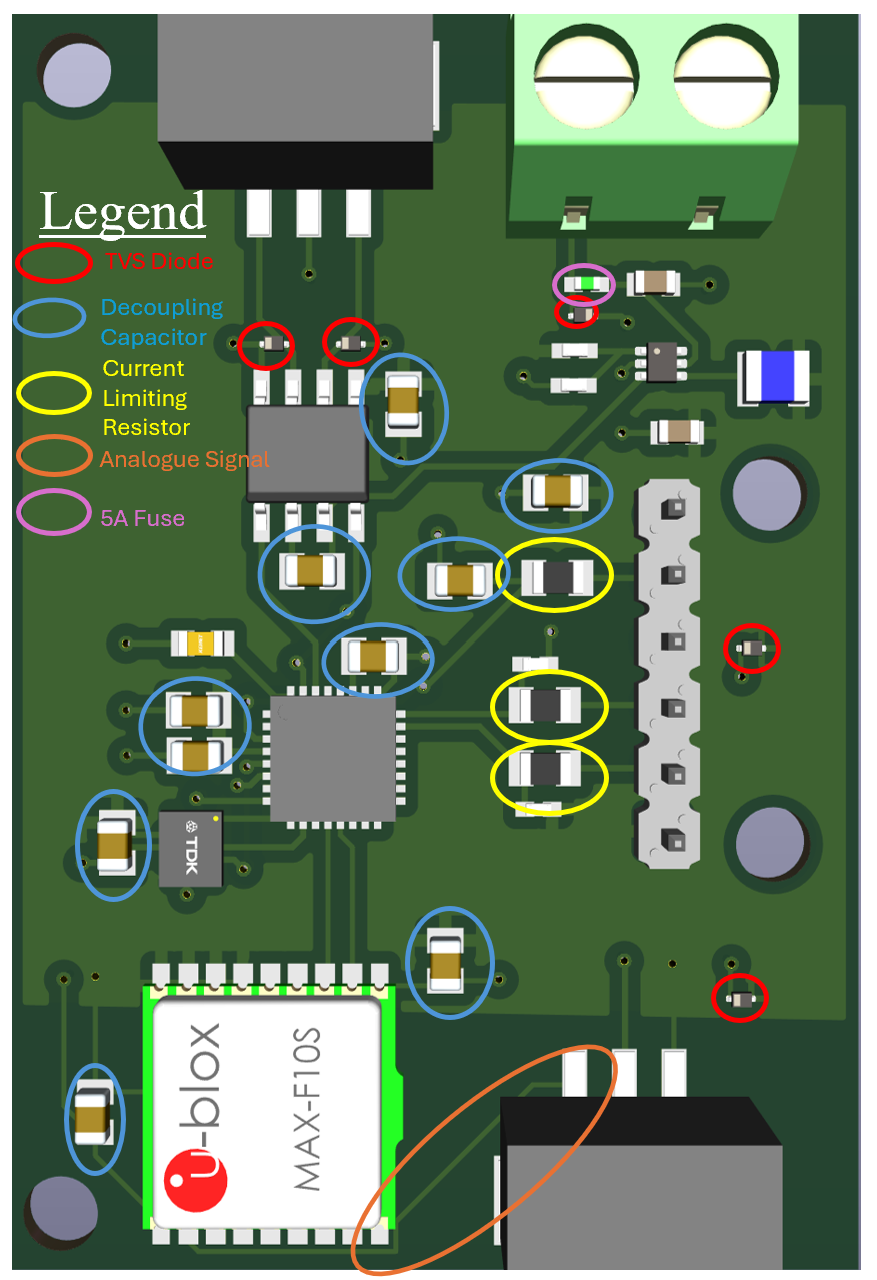
\includegraphics[width=\textwidth]{figs/Thomas/Custom Hardware/GPS render.png}
    \caption{GNSS Module Render}
    \label{fig:gnss_render}
  \end{subfigure}
  \hfill
  \begin{subfigure}[b]{0.48\textwidth}
    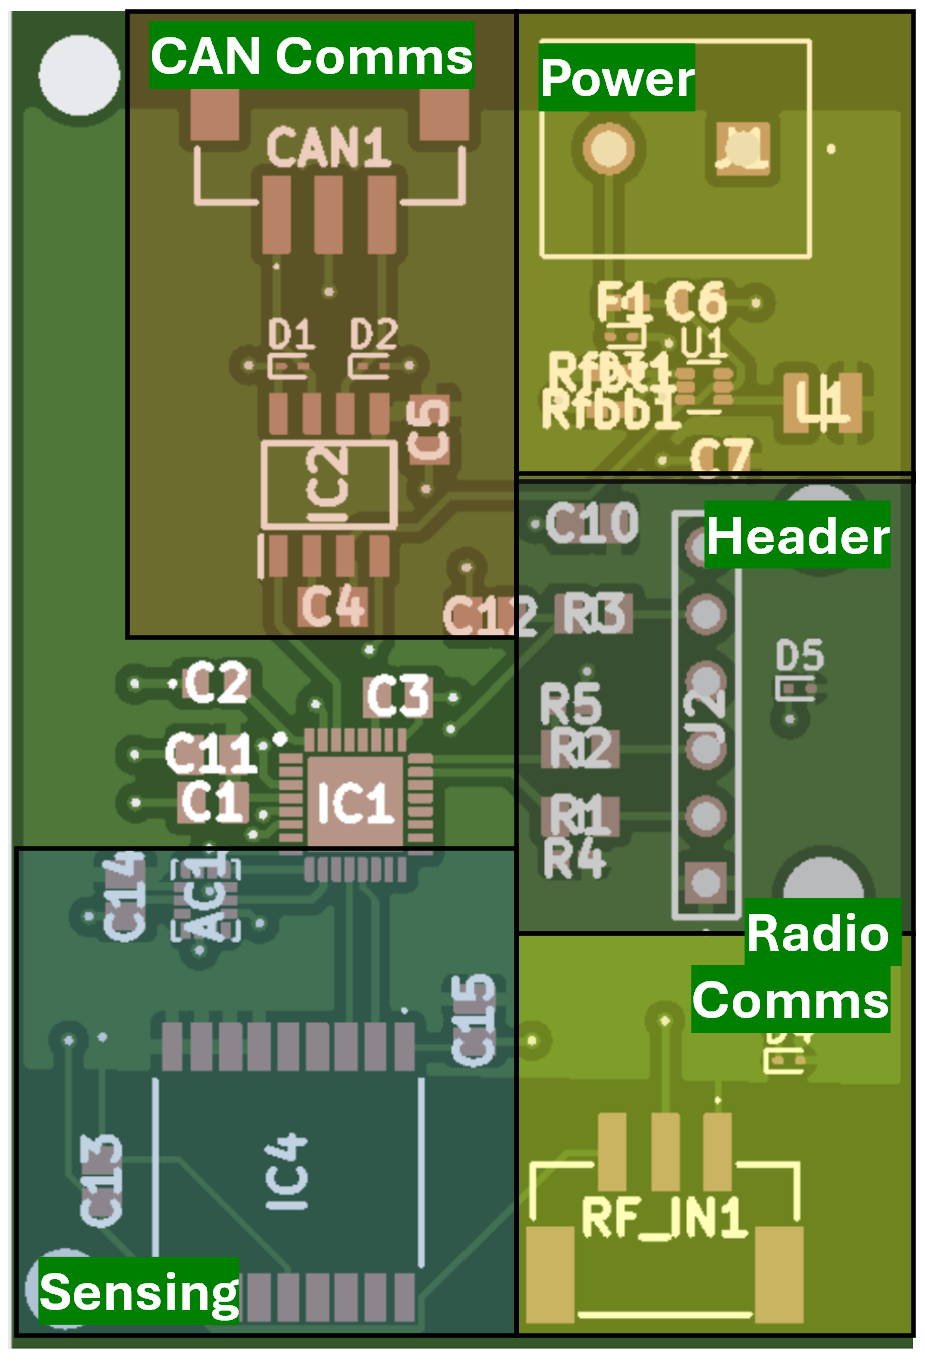
\includegraphics[width=\textwidth]{figs/Thomas/Custom Hardware/GPS gerber.png}
    \caption{GNSS Module Gerber}
    \label{fig:gnss_gerber}
  \end{subfigure}

  
  \begin{subfigure}[b]{0.48\textwidth}
    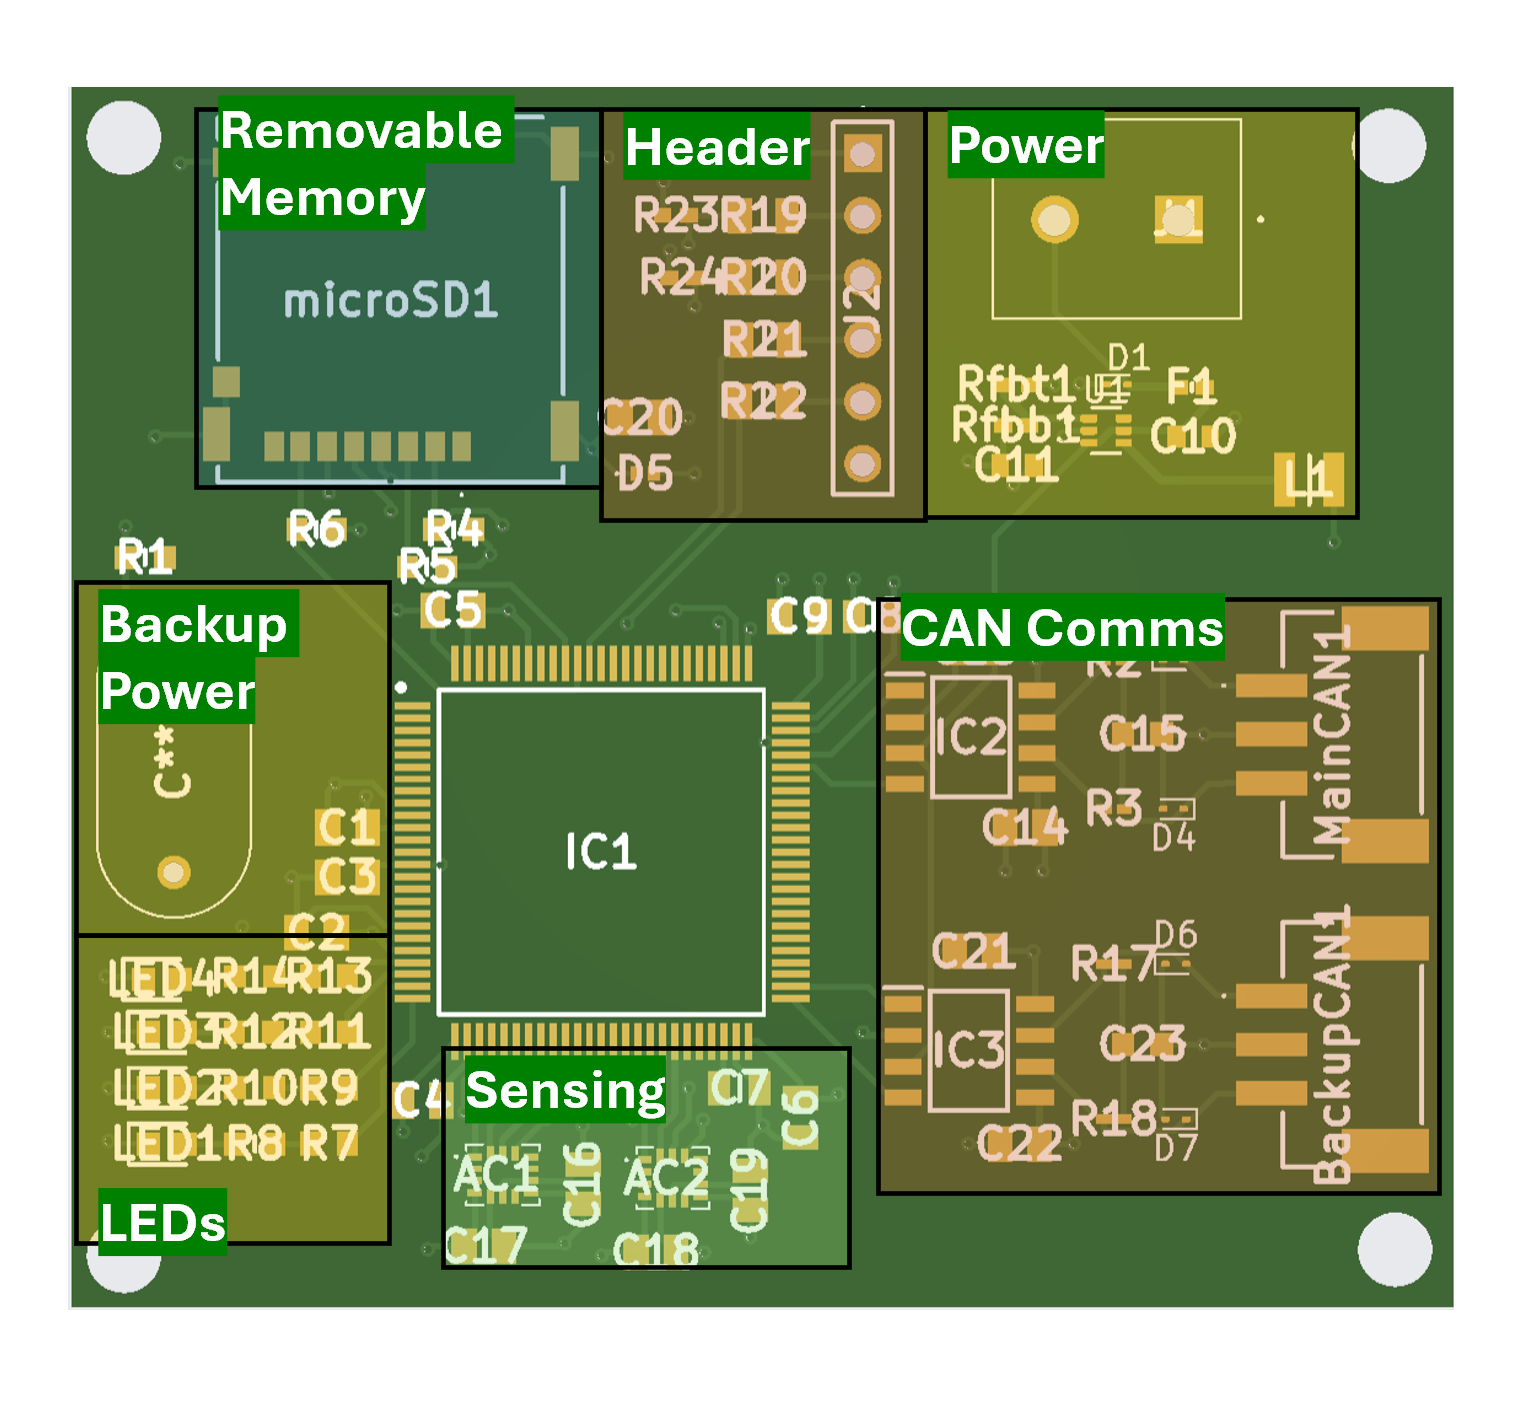
\includegraphics[width=\textwidth]{figs/Thomas/Custom Hardware/FC gerber.png}
    \caption{Custom Flight Controller Gerber}
    \label{fig:fc_gerber}
  \end{subfigure}
  \hfill
  \begin{subfigure}[b]{0.48\textwidth}
    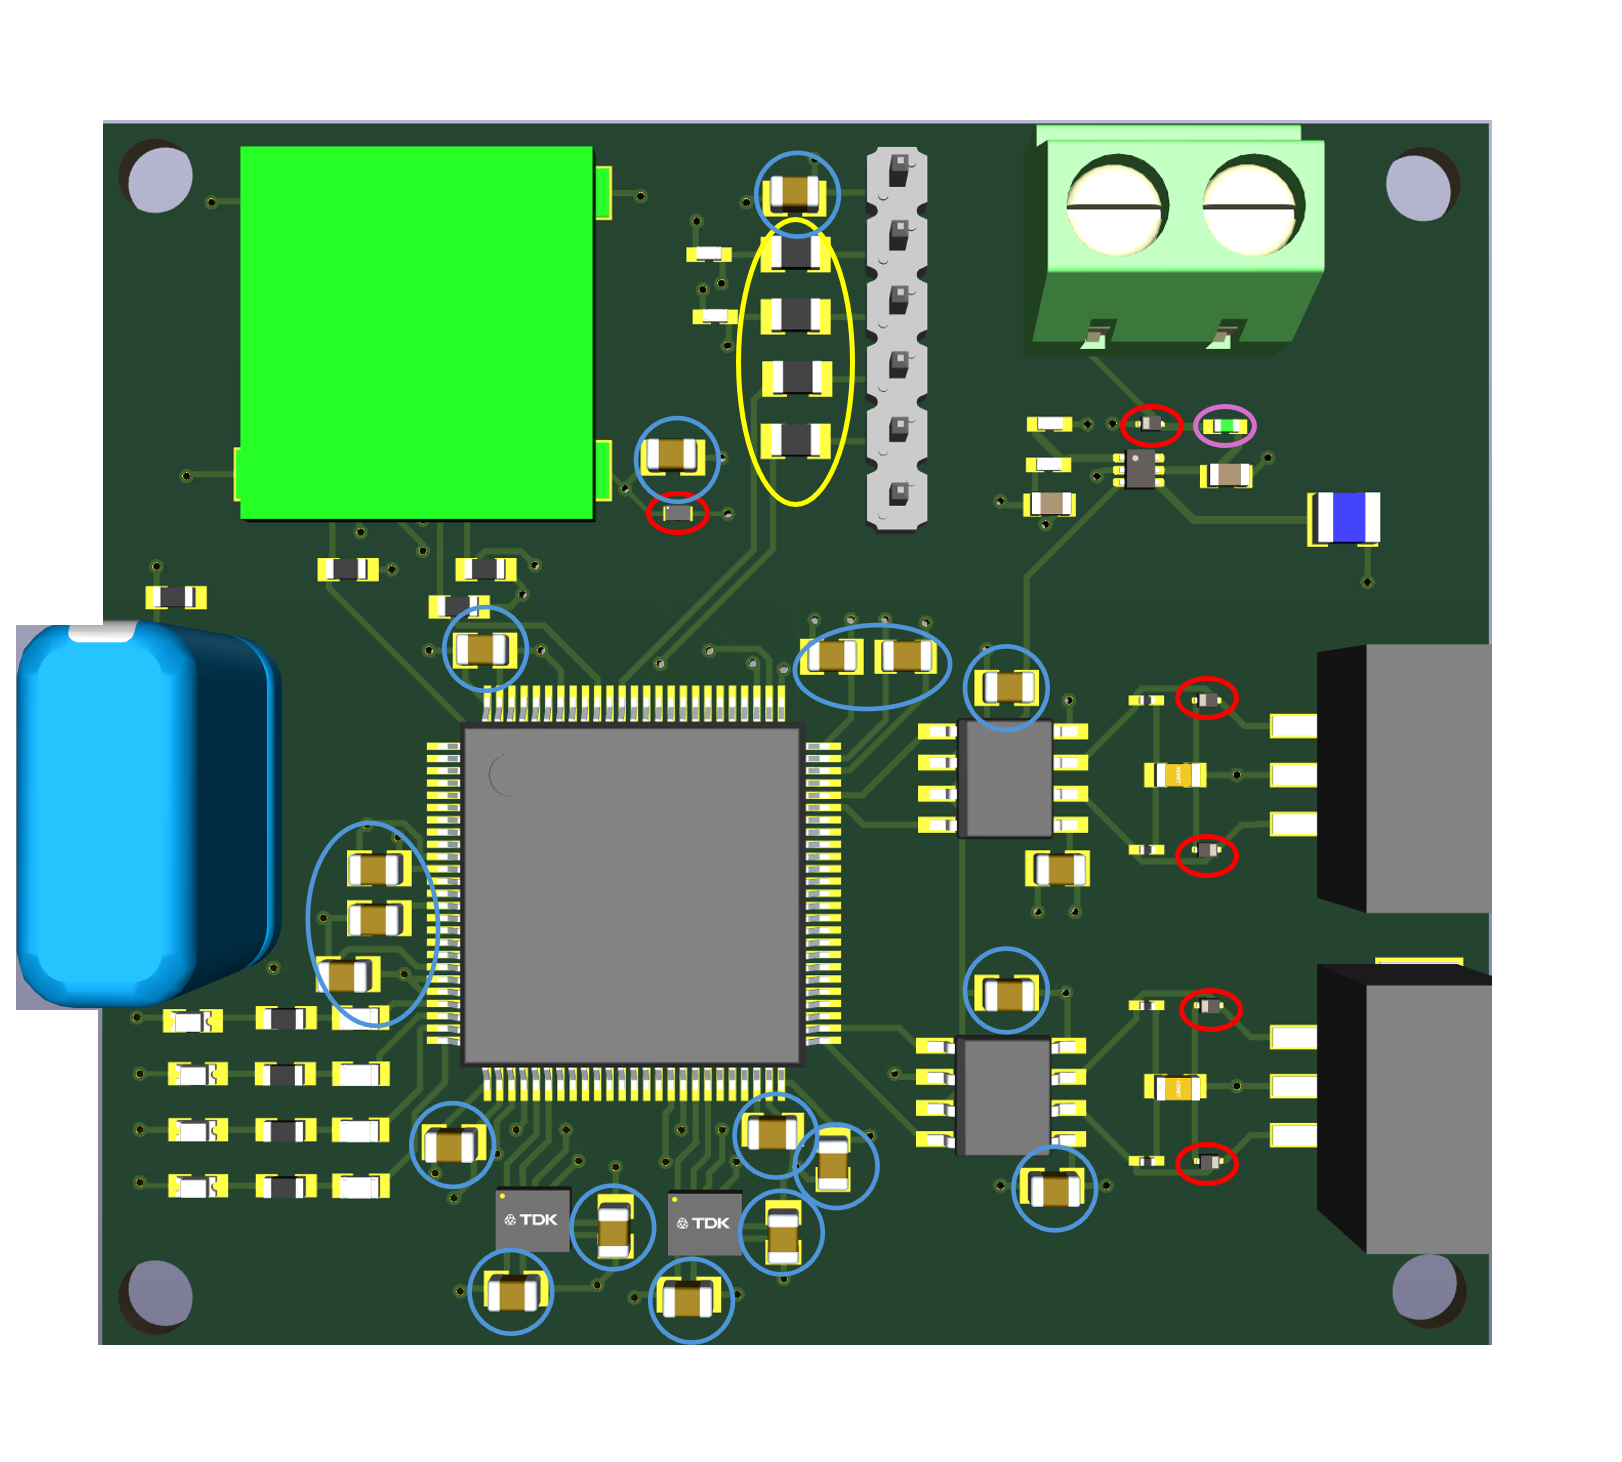
\includegraphics[width=\textwidth]{figs/Thomas/Custom Hardware/FC render.png}
    \caption{Custom Flight Controller Render}
    \label{fig:fc_render}
  \end{subfigure}

  \vspace{1em} % space between rows
  \caption{Custom Hardware Boards: Flight Controller and GNSS Module with Legend}
  \label{fig:custom_hardware_overview}
\end{figure}

